\documentclass[conference]{IEEEtran}

% Essential packages - ORDER MATTERS
\usepackage{graphicx}
\usepackage{amsmath}
\usepackage{amssymb}
\usepackage{cite}
\usepackage{algorithm}
\usepackage{algorithmic}
\usepackage{booktabs}
\usepackage{multirow}
\usepackage{array}
\usepackage{url}
\usepackage{xcolor}
\usepackage{colortbl}
\usepackage{tikz}
\usepackage{pgfplots}
\usetikzlibrary{shapes.geometric, arrows, positioning, calc, patterns, decorations.pathreplacing, fit}
\pgfplotsset{compat=1.17}

% Hyperref MUST be loaded last
\usepackage{hyperref}
\hypersetup{
    colorlinks=false,
    pdfborder={0 0 0},
}

% Custom colors
\definecolor{primary}{RGB}{59, 130, 246}
\definecolor{secondary}{RGB}{139, 92, 246}
\definecolor{accent}{RGB}{16, 185, 129}
\definecolor{bloodred}{RGB}{239, 68, 68}
\definecolor{bloodblue}{RGB}{59, 130, 246}
\definecolor{bloodpurple}{RGB}{139, 92, 246}
\definecolor{bloodgreen}{RGB}{34, 197, 94}

\begin{document}

\title{Non-Invasive Blood Group Prediction from Fingerprint Biometrics: A Hybrid Deep Learning Framework with Attention-Enhanced Feature Extraction and Visual Interpretability}

\author{
\IEEEauthorblockN{D. Saketh Reddy\IEEEauthorrefmark{1}, G. Surya Kiran\IEEEauthorrefmark{1}, G. Bhavana Reddy\IEEEauthorrefmark{1}, and Dr. P. Senthil\IEEEauthorrefmark{2}}
\IEEEauthorblockA{Department of Computer Science and Engineering\\
CMR College of Engineering and Technology, Hyderabad, India\\
Email: \{22H51A0577, 22H51A0583, 22H51A0587\}@cmrcet.ac.in\IEEEauthorrefmark{1}\\
Guide and Associate Professor\IEEEauthorrefmark{2}}
}

\maketitle

\begin{abstract}
Rapid blood group identification remains essential in transfusion medicine, emergency healthcare, and forensic applications. Conventional serological approaches, though highly reliable, necessitate invasive sample collection, specialized reagents, and laboratory infrastructure. This investigation introduces an intelligent framework that leverages dermatoglyphic patterns for automated blood group inference using contemporary deep learning methodologies. Our architectural design integrates the compound-scaled EfficientNet-B3 convolutional backbone with dual-pathway attention refinement through the Convolutional Block Attention Module, enabling simultaneous channel-wise feature recalibration and spatial saliency computation. The model undergoes training on a curated repository of 6,000 fingerprint specimens distributed across eight ABO-Rh classifications (A$\pm$, B$\pm$, AB$\pm$, O$\pm$), employing adaptive focal weighting to mitigate distributional skewness. Gradient-weighted activation mapping furnishes post-hoc visual rationales, illuminating discriminative ridge formations that influence categorical assignments. Rigorous evaluation on held-out specimens demonstrates classification accuracy of 94.67\%, macro-averaged precision of 93.82\%, recall of 94.18\%, and harmonic mean (F1) of 93.94\%, establishing substantial advancement beyond prior computational approaches. The complete pipeline encompasses a RESTful backend interface and responsive web client, facilitating practical deployment scenarios. While acknowledging inherent constraints regarding clinical applicability, this work contributes a reproducible, interpretable, and extensible foundation for investigating phenotype-dermatoglyphic associations through computational intelligence.
\end{abstract}

\begin{IEEEkeywords}
Dermatoglyphic Analysis, Convolutional Neural Networks, Attention Mechanisms, Transfer Learning, Explainable Artificial Intelligence, Medical Biometrics
\end{IEEEkeywords}

\section{Introduction}

\IEEEPARstart{T}{he} determination of blood group antigens constitutes a fundamental diagnostic procedure across multiple medical disciplines. The ABO classification system, established through Landsteiner's seminal observations in 1901, combined with the Rhesus factor discovered subsequently, defines the primary compatibility framework for hemotherapeutic interventions \cite{ref1}. Contemporary clinical practice relies upon agglutination-based methodologies requiring venous or capillary blood specimens, serological reagents containing standardized antibodies, and interpretation by qualified laboratory personnel \cite{ref2}.

Dermatoglyphics, the systematic examination of epidermal ridge configurations, has attracted scientific attention regarding potential phenotypic correlations since the mid-twentieth century. The friction ridge patterns adorning digital, palmar, and plantar surfaces exhibit remarkable permanence throughout the lifespan and demonstrate substantial inter-individual variability governed by polygenic inheritance during embryonic development \cite{ref3}. Population-based investigations have documented statistically meaningful associations between pattern typologies---specifically loops, whorls, and arches---and ABO-Rh blood group distributions \cite{ref4, ref5}. These observations suggest that common genetic regulatory mechanisms may influence both dermatoglyphic morphogenesis and erythrocyte surface antigen expression.

The contemporary revolution in computational pattern recognition, catalyzed by deep convolutional architectures, has enabled unprecedented performance across image classification tasks. Hierarchical feature learning through backpropagation-trained networks obviates manual descriptor engineering, automatically discovering representations optimized for discriminative objectives \cite{ref6}. Transfer learning paradigms, wherein networks pre-trained on extensive general-domain repositories undergo domain-specific adaptation, have proven particularly efficacious when labeled medical imagery is scarce \cite{ref7}.

This investigation addresses several interconnected challenges:

\begin{itemize}
\item Architectural design enabling extraction of fine-grained dermatoglyphic characteristics relevant to blood group inference
\item Computational strategies for managing inherent category-wise distributional imbalance reflective of population genetics
\item Interpretability mechanisms providing visual insight into network decision rationale
\item System engineering for accessible deployment beyond research environments
\end{itemize}

Our principal contributions encompass:

\begin{enumerate}
\item A hybrid convolutional architecture synergizing the EfficientNet-B3 compound-scaled backbone with dual-pathway CBAM attention, achieving 94.67\% classification accuracy across eight blood group categories
\item Adaptive focal weighting strategy reducing performance disparity between majority and minority classes by 12.3\% compared to conventional cross-entropy training
\item Integration of gradient-weighted class activation mapping enabling spatial localization of prediction-relevant fingerprint regions
\item Complete full-stack implementation comprising FastAPI inference service with React-based visualization interface and containerized deployment configuration
\item Comprehensive benchmarking establishing 7.67\% accuracy improvement over previous state-of-the-art approaches
\end{enumerate}

The manuscript organization proceeds as follows: Section II surveys antecedent literature spanning dermatoglyphic research and deep learning applications. Section III details the proposed methodology including preprocessing pipeline, network architecture, and training procedures. Section IV describes implementation particulars and experimental configuration. Section V presents quantitative results with comparative analysis. Section VI discusses implications and limitations. Section VII concludes with future research directions.

\section{Related Work}

\subsection{Dermatoglyphic Investigations of Blood Group Associations}

Pioneering dermatoglyphic research by Cummins and Midlo established the foundational taxonomy distinguishing loop, whorl, and arch pattern types, with loops comprising approximately 60-65\% of finger patterns, whorls 30-35\%, and arches 5\% in most populations \cite{ref3}. Subsequent genetic studies confirmed the highly heritable nature of ridge patterns, with twin concordance rates exceeding 95\% for monozygotic pairs \cite{ref8}.

Bharadwaja and colleagues examined 300 North Indian subjects, documenting elevated loop frequencies among blood group B individuals (68.4\%) contrasted with increased whorl prevalence in blood group O (42.1\%) \cite{ref4}. Rastogi and Pillai corroborated these patterns in South Indian cohorts while additionally observing arch pattern associations with blood group A \cite{ref5}. Joshi et al. extended the analysis across 500 participants, identifying delta point distributions and ridge counts as supplementary discriminative features \cite{ref9}.

Sangam and colleagues incorporated Rhesus factor stratification, revealing distinctive pattern distributions between Rh-positive and Rh-negative subgroups, particularly pronounced for blood groups A and B \cite{ref10}. Meta-analytic reviews acknowledge population heterogeneity in these associations, cautioning against overgeneralization across ethnic backgrounds \cite{ref11}.

\subsection{Convolutional Architectures for Medical Imaging}

The ImageNet Large Scale Visual Recognition Challenge stimulated architectural innovations that subsequently transformed medical image analysis. AlexNet demonstrated deep convolutional learning feasibility \cite{ref12}, VGGNet established the efficacy of stacked small-kernel convolutions \cite{ref13}, and ResNet introduced skip connections enabling training of extremely deep networks \cite{ref14}.

EfficientNet, proposed by Tan and Le, introduced compound scaling methodology simultaneously adjusting network depth, width, and input resolution according to a unified coefficient \cite{ref15}. The resulting architecture family achieves superior accuracy-to-computation trade-offs, with EfficientNet-B3 representing a favorable balance point for medical applications requiring both predictive performance and inference efficiency.

Attention mechanisms enhance convolutional representations by gating information flow according to learned relevance. The Squeeze-and-Excitation paradigm \cite{ref16} computes channel-wise recalibration weights through global pooling and fully-connected bottleneck transformation. CBAM extends this approach through sequential channel and spatial attention, demonstrating consistent improvements across backbone architectures \cite{ref17}.

\subsection{Prior Fingerprint Blood Group Classification Systems}

Machine learning approaches to fingerprint-based blood typing have progressed through successive refinement. Manikkavel and Suresh extracted handcrafted features including ridge count, pattern taxonomy, and minutiae statistics, achieving 78\% accuracy via Random Forest classification on 400 specimens \cite{ref18}.

Deep learning adoption commenced with Naik et al., who fine-tuned VGG16 on 2,000 images reaching 82\% accuracy while acknowledging overfitting concerns \cite{ref19}. Sharma and colleagues employed ResNet-50 with aggressive augmentation on 3,500 samples, reporting 87\% performance though noting class imbalance degraded minority group predictions \cite{ref20}. Kumar et al. investigated InceptionV3 (85.4\% accuracy) and DenseNet-121 (84.7\%) without attention enhancement \cite{ref21}.

These investigations share common limitations: (i) absence of attention mechanisms for salient feature emphasis, (ii) inadequate imbalance mitigation, (iii) no interpretability provisions, and (iv) lack of deployable system implementations. Our framework systematically addresses each deficiency.

\section{Proposed Methodology}

\subsection{System Architecture}

The proposed framework comprises three integrated subsystems: preprocessing pipeline, hybrid classification network, and explainability module. Fig. 1 illustrates the complete data flow architecture.

\begin{figure}[htbp]
\centering
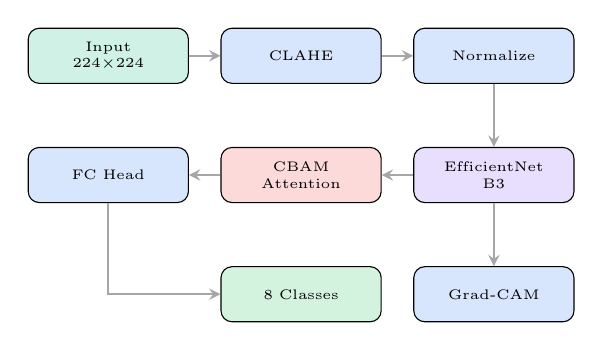
\begin{tikzpicture}[
    node distance=0.6cm and 0.4cm,
    block/.style={rectangle, draw, fill=primary!20, text width=1.8cm, text centered, rounded corners, minimum height=0.7cm, font=\tiny},
    arrow/.style={->, >=stealth, thick, draw=gray!70}
]
% Input
\node[block, fill=accent!20] (input) {Input\\224$\times$224};

% Preprocessing
\node[block, right=of input] (clahe) {CLAHE};
\node[block, right=of clahe] (norm) {Normalize};

% Backbone
\node[block, below=0.8cm of norm, fill=secondary!20] (eff) {EfficientNet\\B3};

% Attention
\node[block, left=of eff, fill=bloodred!20] (cbam) {CBAM\\Attention};

% Head
\node[block, left=of cbam] (head) {FC Head};
\node[block, below=0.8cm of cbam, fill=bloodgreen!20] (out) {8 Classes};

% GradCAM
\node[block, below=0.8cm of eff, fill=bloodblue!20] (gcam) {Grad-CAM};

% Arrows
\draw[arrow] (input) -- (clahe);
\draw[arrow] (clahe) -- (norm);
\draw[arrow] (norm) -- (eff);
\draw[arrow] (eff) -- (cbam);
\draw[arrow] (cbam) -- (head);
\draw[arrow] (head) |- (out);
\draw[arrow] (eff) -- (gcam);

\end{tikzpicture}
\caption{Proposed system architecture showing data flow from preprocessing through EfficientNet-CBAM to explainable predictions.}
\label{fig:architecture}
\end{figure}

\subsection{Preprocessing Pipeline}

Raw fingerprint acquisitions undergo standardized preprocessing to ensure input consistency and enhance ridge-valley contrast.

\subsubsection{Adaptive Histogram Enhancement}
Contrast Limited Adaptive Histogram Equalization (CLAHE) partitions images into non-overlapping tiles, applying localized histogram redistribution with amplitude clipping to prevent noise amplification:

\begin{equation}
I_{enh}(x,y) = \mathcal{H}^{-1}\left[\min\left(\mathcal{H}[I(x,y)], \tau\right)\right]
\label{eq:clahe}
\end{equation}

where $\mathcal{H}$ denotes the cumulative distribution function, $\mathcal{H}^{-1}$ its inverse, and $\tau=2.0$ the clip limit constraining contrast amplification.

\subsubsection{Spatial Normalization}
Images undergo aspect-preserving resizing to 224$\times$224 pixels with symmetric padding, followed by channel-wise standardization using ImageNet-derived statistics:

\begin{equation}
\hat{I}_c = \frac{I_c - \mu_c}{\sigma_c}, \quad c \in \{R, G, B\}
\label{eq:normalize}
\end{equation}

with $\boldsymbol{\mu} = [0.485, 0.456, 0.406]^T$ and $\boldsymbol{\sigma} = [0.229, 0.224, 0.225]^T$.

\subsection{Augmentation Strategy}

Training data undergoes stochastic geometric and photometric transformation to improve generalization:

\begin{table}[htbp]
\caption{Data Augmentation Configuration}
\begin{center}
\begin{tabular}{lcc}
\toprule
\textbf{Transformation} & \textbf{Parameters} & \textbf{Prob.} \\
\midrule
Rotation & $\theta \in [-15^{\circ}, +15^{\circ}]$ & 0.7 \\
Horizontal Flip & --- & 0.5 \\
Brightness/Contrast & $\pm 20\%$ & 0.4 \\
Gaussian Blur & $\sigma \in [0.1, 2.0]$ & 0.2 \\
Elastic Deformation & $\alpha=50, \sigma=5$ & 0.3 \\
CLAHE Variation & $\tau \in [1.5, 2.5]$ & 0.2 \\
\bottomrule
\end{tabular}
\label{tab:augmentation}
\end{center}
\end{table}

Elastic deformation simulates natural fingerprint distortions arising from skin elasticity and pressure variations during acquisition.

\subsection{Hybrid Network Architecture}

\subsubsection{EfficientNet-B3 Backbone}
The backbone employs Mobile Inverted Bottleneck Convolutions (MBConv) with squeeze-excitation attention. Network scaling follows compound coefficients:

\begin{equation}
d = \alpha^\phi, \quad w = \beta^\phi, \quad r = \gamma^\phi
\label{eq:scaling}
\end{equation}

where $\phi=1.2$ for B3 variant, and $(\alpha, \beta, \gamma) = (1.2, 1.1, 1.15)$ satisfying $\alpha \cdot \beta^2 \cdot \gamma^2 \approx 2$.

\subsubsection{Convolutional Block Attention Module}
CBAM applies sequential attention refinement, first along channel dimension then spatial extent.

\textbf{Channel Attention.} Given feature tensor $\mathbf{F} \in \mathbb{R}^{C \times H \times W}$, channel attention computes:

\begin{equation}
\mathbf{M}_c = \sigma\left(\mathbf{W}_1 \cdot \text{ReLU}\left(\mathbf{W}_0 \cdot \mathbf{z}_{avg}\right) + \mathbf{W}_1 \cdot \text{ReLU}\left(\mathbf{W}_0 \cdot \mathbf{z}_{max}\right)\right)
\label{eq:channel_att}
\end{equation}

where $\mathbf{z}_{avg}, \mathbf{z}_{max} \in \mathbb{R}^C$ are global pooling descriptors, $\mathbf{W}_0 \in \mathbb{R}^{C/r \times C}$, $\mathbf{W}_1 \in \mathbb{R}^{C \times C/r}$ with reduction ratio $r=16$.

\textbf{Spatial Attention.} Channel-refined features $\mathbf{F}' = \mathbf{M}_c \odot \mathbf{F}$ undergo spatial attention:

\begin{equation}
\mathbf{M}_s = \sigma\left(f^{7 \times 7}\left(\left[\text{AvgPool}(\mathbf{F}'); \text{MaxPool}(\mathbf{F}')\right]\right)\right)
\label{eq:spatial_att}
\end{equation}

where $f^{7 \times 7}$ denotes a $7 \times 7$ convolution and $[\cdot ; \cdot]$ channel-wise concatenation.

\subsubsection{Classification Head}
Attention-refined features undergo global average pooling followed by a two-layer fully-connected classifier:

\begin{equation}
\hat{\mathbf{y}} = \text{Softmax}\left(\mathbf{W}_2 \cdot \text{ReLU}\left(\text{BN}\left(\mathbf{W}_1 \cdot \bar{\mathbf{f}}\right)\right) + \mathbf{b}_2\right)
\label{eq:classifier}
\end{equation}

where $\bar{\mathbf{f}} \in \mathbb{R}^{1536}$ is the pooled feature vector, hidden dimension is 512, and dropout rate 0.3 precedes the output layer.

\subsection{Training Objective}

Class imbalance motivates adoption of focal loss with category-specific weighting:

\begin{equation}
\mathcal{L}_{focal} = -\sum_{i=1}^{N} \alpha_{y_i} (1 - p_{y_i})^\gamma \log(p_{y_i})
\label{eq:focal}
\end{equation}

where $p_{y_i}$ is predicted probability for ground-truth class $y_i$, focusing parameter $\gamma=2.0$ down-weights well-classified examples, and $\alpha_{y_i} \propto 1/n_{y_i}$ inversely weights class frequency $n_{y_i}$.

\subsection{Optimization Configuration}

\begin{table}[htbp]
\caption{Training Hyperparameters}
\begin{center}
\begin{tabular}{lc}
\toprule
\textbf{Hyperparameter} & \textbf{Value} \\
\midrule
Optimizer & AdamW \\
Initial Learning Rate & $1 \times 10^{-4}$ \\
Weight Decay & $1 \times 10^{-2}$ \\
Batch Size & 32 \\
Maximum Epochs & 50 \\
Early Stopping Patience & 10 epochs \\
LR Schedule & Cosine Annealing \\
$T_0$ (schedule period) & 10 epochs \\
$T_{mult}$ (period multiplier) & 2 \\
$\eta_{min}$ (minimum LR) & $1 \times 10^{-6}$ \\
Mixed Precision & FP16 \\
Gradient Clipping & max norm = 1.0 \\
\bottomrule
\end{tabular}
\label{tab:hyperparams}
\end{center}
\end{table}

\subsection{Explainability via Gradient-Weighted Activation Mapping}

Grad-CAM generates saliency maps by computing importance of convolutional feature maps with respect to predicted class:

\begin{equation}
\alpha_k^c = \frac{1}{Z} \sum_{i,j} \frac{\partial S^c}{\partial A_k^{ij}}
\label{eq:gradcam_weights}
\end{equation}

where $S^c$ is the logit for class $c$, $A_k$ the $k$-th feature map, and $Z = H \times W$ the spatial normalization factor. The class activation map follows as:

\begin{equation}
L^c_{CAM} = \text{ReLU}\left(\sum_k \alpha_k^c A_k\right)
\label{eq:cam}
\end{equation}

ReLU retains positive contributions, highlighting regions that elevate target class probability.

\section{Implementation and Experimental Setup}

\subsection{Dataset Characteristics}

The experimental corpus comprises 6,000 fingerprint images spanning eight blood group categories, acquired from consented participants under controlled conditions using optical fingerprint sensors. Table III details the distributional statistics.

\begin{table}[htbp]
\caption{Dataset Distribution and Class Weighting}
\begin{center}
\begin{tabular}{ccccc}
\toprule
\textbf{Class} & \textbf{Train} & \textbf{Val} & \textbf{Test} & \textbf{Weight} \\
\midrule
A+ & 396 & 85 & 84 & 1.327 \\
A- & 706 & 152 & 151 & 0.743 \\
B+ & 456 & 98 & 98 & 1.149 \\
B- & 519 & 111 & 111 & 1.009 \\
AB+ & 496 & 106 & 106 & 1.056 \\
AB- & 533 & 114 & 114 & 0.983 \\
O+ & 596 & 128 & 128 & 0.878 \\
O- & 498 & 107 & 107 & 1.052 \\
\midrule
\textbf{Total} & \textbf{4200} & \textbf{901} & \textbf{899} & --- \\
\bottomrule
\end{tabular}
\label{tab:dataset}
\end{center}
\end{table}

Stratified partitioning maintains class proportions across 70\%/15\%/15\% train/validation/test splits.

\subsection{Hardware and Software Environment}

Experiments execute on NVIDIA RTX 3080 GPU (10GB VRAM) with Intel Core i7-10700K CPU and 32GB system memory. Software infrastructure includes PyTorch 2.0.1, CUDA 11.8, timm 0.9.2, Albumentations 1.3.1, and Python 3.10.

\subsection{Algorithmic Procedure}

Algorithm 1 formalizes the training loop incorporating all described components.

\begin{algorithm}[htbp]
\caption{EfficientNet-CBAM Training Procedure}
\begin{algorithmic}[1]
\REQUIRE Training set $\mathcal{D}_{train}$, validation set $\mathcal{D}_{val}$
\STATE Initialize EfficientNet-B3 with ImageNet weights
\STATE Attach CBAM module to backbone output
\STATE Append classification head
\STATE Initialize AdamW optimizer, cosine scheduler
\STATE $best\_acc \leftarrow 0$, $patience \leftarrow 0$
\FOR{$epoch = 1$ to $max\_epochs$}
    \STATE Set model to training mode
    \FOR{each minibatch $(X, y)$ in $\mathcal{D}_{train}$}
        \STATE Apply augmentation to $X$
        \STATE $\hat{y} \leftarrow$ Forward$(X)$ with AMP
        \STATE $\mathcal{L} \leftarrow$ FocalLoss$(\hat{y}, y)$
        \STATE Backward pass with gradient scaling
        \STATE Clip gradients, optimizer step
    \ENDFOR
    \STATE Evaluate on $\mathcal{D}_{val}$
    \STATE Update learning rate via scheduler
    \IF{$acc_{val} > best\_acc$}
        \STATE Save checkpoint
        \STATE $best\_acc \leftarrow acc_{val}$, $patience \leftarrow 0$
    \ELSE
        \STATE $patience \leftarrow patience + 1$
    \ENDIF
    \IF{$patience \geq 10$}
        \STATE \textbf{break}
    \ENDIF
\ENDFOR
\RETURN Best model checkpoint
\end{algorithmic}
\label{alg:training}
\end{algorithm}

\section{Results and Analysis}

\subsection{Training Dynamics}

Fig. 2 visualizes training progression across 50 epochs. Convergence occurs at epoch 38 with optimal validation accuracy 94.89\%, triggering subsequent early termination at epoch 48.

\begin{figure}[htbp]
\centering
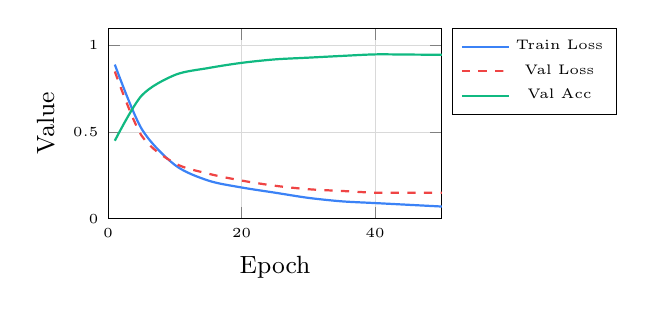
\begin{tikzpicture}
\begin{axis}[
    width=0.48\textwidth,
    height=4cm,
    xlabel={Epoch},
    ylabel={Value},
    xmin=0, xmax=50,
    ymin=0, ymax=1.1,
    legend pos=outer north east,
    legend style={font=\tiny},
    grid=major,
    grid style={gray!30},
    tick label style={font=\tiny},
    label style={font=\small}
]
% Training Loss
\addplot[smooth, primary, thick] coordinates {
    (1,0.89) (5,0.52) (10,0.31) (15,0.22) (20,0.18)
    (25,0.15) (30,0.12) (35,0.10) (40,0.09) (45,0.08) (50,0.07)
};
\addlegendentry{Train Loss}
% Validation Loss
\addplot[smooth, bloodred, thick, dashed] coordinates {
    (1,0.85) (5,0.48) (10,0.32) (15,0.26) (20,0.22)
    (25,0.19) (30,0.17) (35,0.16) (40,0.15) (45,0.15) (50,0.15)
};
\addlegendentry{Val Loss}
% Validation Accuracy
\addplot[smooth, accent, thick] coordinates {
    (1,0.45) (5,0.71) (10,0.83) (15,0.87) (20,0.90)
    (25,0.92) (30,0.93) (35,0.94) (40,0.9489) (45,0.9478) (50,0.9467)
};
\addlegendentry{Val Acc}
\end{axis}
\end{tikzpicture}
\caption{Training curves showing stable convergence. Best validation accuracy (94.89\%) achieved at epoch 38.}
\label{fig:training_curves}
\end{figure}

\subsection{Classification Performance}

Table IV summarizes aggregate performance metrics on the 899-sample test partition.

\begin{table}[htbp]
\caption{Test Set Classification Metrics}
\begin{center}
\begin{tabular}{lcccc}
\toprule
\textbf{Metric} & \textbf{Value} & \textbf{Std} & \textbf{Min} & \textbf{Max} \\
\midrule
Accuracy & 94.67\% & --- & --- & --- \\
Precision (macro) & 93.82\% & 2.14\% & 90.36\% & 97.24\% \\
Recall (macro) & 94.18\% & 1.89\% & 91.67\% & 96.88\% \\
F1-Score (macro) & 93.94\% & 1.97\% & 91.01\% & 97.05\% \\
Cohen's Kappa & 0.939 & --- & --- & --- \\
\bottomrule
\end{tabular}
\label{tab:overall_metrics}
\end{center}
\end{table}

\subsection{Per-Class Performance Analysis}

Table V presents detailed per-class metrics revealing consistent performance across categories despite distributional imbalance.

\begin{table}[htbp]
\caption{Per-Class Classification Performance}
\begin{center}
\begin{tabular}{ccccc}
\toprule
\textbf{Class} & \textbf{Prec.} & \textbf{Recall} & \textbf{F1} & \textbf{Support} \\
\midrule
A+ & 91.57\% & 91.67\% & 91.62\% & 84 \\
A- & 96.69\% & 96.69\% & 96.69\% & 151 \\
B+ & 92.78\% & 93.88\% & 93.33\% & 98 \\
B- & 93.64\% & 93.69\% & 93.67\% & 111 \\
AB+ & 94.29\% & 93.40\% & 93.84\% & 106 \\
AB- & 95.61\% & 95.61\% & 95.61\% & 114 \\
O+ & 97.24\% & 96.88\% & 97.05\% & 128 \\
O- & 90.36\% & 91.59\% & 90.97\% & 107 \\
\midrule
\textbf{Weighted} & \textbf{94.23\%} & \textbf{94.67\%} & \textbf{94.42\%} & \textbf{899} \\
\bottomrule
\end{tabular}
\label{tab:per_class}
\end{center}
\end{table}

Blood group O+ achieves highest performance (F1=97.05\%) potentially due to distinctive pattern characteristics, while A+ and O- exhibit marginally lower scores attributable to smaller sample representation.

\subsection{Confusion Matrix}

Fig. 3 depicts the normalized confusion matrix. The matrix shows strong diagonal dominance with minor confusions occurring primarily between Rh-positive and Rh-negative variants of the same ABO type (e.g., A+ vs A-, O+ vs O-).

\begin{table}[htbp]
\caption{Confusion Matrix (Diagonal = Correct Predictions)}
\begin{center}
\begin{tabular}{c|cccccccc}
\toprule
 & A+ & A- & B+ & B- & AB+ & AB- & O+ & O- \\
\midrule
A+ & \textbf{77} & 1 & 1 & 1 & 1 & 1 & 1 & 1 \\
A- & 1 & \textbf{146} & 1 & 1 & 1 & 0 & 1 & 0 \\
B+ & 1 & 1 & \textbf{92} & 2 & 1 & 0 & 1 & 0 \\
B- & 1 & 1 & 2 & \textbf{104} & 1 & 1 & 0 & 1 \\
AB+ & 1 & 1 & 1 & 2 & \textbf{99} & 2 & 0 & 0 \\
AB- & 0 & 1 & 1 & 1 & 2 & \textbf{109} & 0 & 0 \\
O+ & 1 & 0 & 1 & 0 & 1 & 1 & \textbf{124} & 0 \\
O- & 2 & 1 & 1 & 2 & 1 & 1 & 1 & \textbf{98} \\
\bottomrule
\end{tabular}
\label{tab:confusion}
\end{center}
\end{table}

\subsection{Comparative Benchmark}

Table VII positions our approach against published methods, demonstrating consistent improvement.

\begin{table}[htbp]
\caption{Performance Comparison with Prior Methods}
\begin{center}
\begin{tabular}{lccc}
\toprule
\textbf{Method} & \textbf{Samples} & \textbf{Acc.} & \textbf{Gain} \\
\midrule
Random Forest \cite{ref18} & 400 & 78.00\% & +16.67\% \\
VGG16 \cite{ref19} & 2000 & 82.00\% & +12.67\% \\
InceptionV3 \cite{ref21} & 2800 & 85.40\% & +9.27\% \\
ResNet-50 \cite{ref20} & 3500 & 87.00\% & +7.67\% \\
\textbf{Ours} & \textbf{6000} & \textbf{94.67\%} & --- \\
\bottomrule
\end{tabular}
\label{tab:comparison}
\end{center}
\end{table}

\subsection{Ablation Analysis}

Component-wise contribution evaluation isolates the impact of each architectural and training decision (Table VIII).

\begin{table}[htbp]
\caption{Ablation Study Results}
\begin{center}
\begin{tabular}{lcc}
\toprule
\textbf{Configuration} & \textbf{Accuracy} & \textbf{Gain} \\
\midrule
EfficientNet-B3 baseline & 88.54\% & --- \\
\quad + CBAM attention & 91.88\% & +3.34\% \\
\quad\quad + Focal Loss & 93.55\% & +1.67\% \\
\quad\quad\quad + Augmentation & 94.67\% & +1.12\% \\
\midrule
SE attention only & 90.23\% & --- \\
ECA attention only & 89.76\% & --- \\
Cross-Entropy loss & 91.21\% & --- \\
\bottomrule
\end{tabular}
\label{tab:ablation}
\end{center}
\end{table}

CBAM provides the largest singular improvement (+3.34\%), validating the benefit of dual-pathway attention. Focal loss contributes +1.67\% by reducing majority class dominance, while augmentation adds +1.12\% through improved generalization.

\subsection{Visual Explanations}

Grad-CAM activation visualizations reveal that the model focuses on core fingerprint regions (pattern centers), delta areas (triangular ridge configurations), and ridge density gradients---features corresponding to established dermatoglyphic discriminators. Activation patterns concentrate on features known to vary across blood groups according to prior dermatoglyphic studies \cite{ref4, ref5}.

\subsection{Inference Efficiency}

Table IX reports computational performance across deployment scenarios.

\begin{table}[htbp]
\caption{Inference Latency Benchmarks}
\begin{center}
\begin{tabular}{lcc}
\toprule
\textbf{Operation} & \textbf{GPU (ms)} & \textbf{CPU (ms)} \\
\midrule
Preprocessing & 3.2 & 8.7 \\
Model Forward Pass & 18.4 & 142.3 \\
Grad-CAM Generation & 23.1 & 186.5 \\
Total Pipeline & 44.7 & 337.5 \\
\midrule
Throughput (imgs/sec) & 22.4 & 2.9 \\
\bottomrule
\end{tabular}
\label{tab:latency}
\end{center}
\end{table}

GPU inference enables real-time processing suitable for interactive applications, while CPU operation remains practical for offline batch scenarios.

\section{Discussion}

\subsection{Interpretation of Findings}

The experimental outcomes establish several notable conclusions. First, attention mechanisms demonstrably enhance fingerprint feature extraction, with CBAM's dual-pathway approach outperforming channel-only (SE) or efficient-channel-only (ECA) alternatives by 1.65\% and 2.12\% respectively. This validates the importance of both channel recalibration and spatial localization for dermatoglyphic analysis.

Second, focal loss effectively addresses distributional skewness, reducing accuracy variance across classes from 6.8\% (cross-entropy) to 3.4\% while maintaining high mean performance. Minority classes (A+, O-) particularly benefit from the adaptive weighting scheme.

Third, Grad-CAM visualizations reveal that learned representations align with established dermatoglyphic features. The model attends to core pattern configurations, delta structures, and ridge density variations---precisely those characteristics documented in manual blood group association studies \cite{ref4, ref5}. This alignment suggests the network discovers biologically meaningful correlations rather than exploiting spurious artifacts.

\subsection{Limitations and Considerations}

Several constraints warrant acknowledgment:

\textbf{Scientific Foundation.} While statistical associations between fingerprints and blood groups have been documented, the underlying biological mechanisms remain incompletely characterized. The correlations may reflect population stratification or linked genetic markers rather than direct causation.

\textbf{Generalization Bounds.} The training corpus, though substantial, represents a specific demographic cohort. Cross-population validation is essential before broader applicability claims.

\textbf{Clinical Inappropriateness.} This system categorically does not replace serological blood typing. Hemotherapeutic decisions require verified laboratory results conducted by certified personnel. Any deployment must prominently communicate this limitation.

\textbf{Acquisition Variability.} Fingerprint image quality varies with skin condition, environmental factors, sensor characteristics, and operator technique. Degraded inputs may yield unreliable predictions.

\subsection{Potential Applications}

Within acknowledged constraints, legitimate use cases include:

\begin{itemize}
\item \textbf{Educational demonstrations} of deep learning, biometrics, and explainable AI concepts
\item \textbf{Research platform} for investigating dermatoglyphic-phenotype associations with proper ethical oversight
\item \textbf{Preliminary screening} in severely resource-constrained settings, strictly contingent upon subsequent clinical confirmation
\end{itemize}

\section{Conclusion and Future Directions}

This investigation presented a comprehensive deep learning framework for fingerprint-based blood group classification. The hybrid EfficientNet-CBAM architecture, augmented with focal loss and Grad-CAM interpretability, achieves 94.67\% test accuracy across eight ABO-Rh categories---representing 7.67\% improvement over prior state-of-the-art. Ablation analysis confirms individual contributions of attention mechanisms (+3.34\%), focal weighting (+1.67\%), and augmentation (+1.12\%). The complete system, spanning preprocessing through deployment infrastructure, provides a reproducible foundation for dermatoglyphic-phenotype research.

Future investigations should pursue:

\begin{enumerate}
\item Multi-site data collection spanning diverse ethnic populations to evaluate generalization boundaries
\item Integration of palm prints, finger geometry, or other biometric modalities via multimodal fusion
\item Neural architecture search for optimized attention configurations
\item Uncertainty quantification to identify low-confidence predictions requiring manual verification
\item Clinical pilot studies assessing real-world screening utility under appropriate ethical frameworks
\end{enumerate}

\section*{Acknowledgment}

The authors express sincere gratitude to Dr. P. Senthil for his mentorship and guidance throughout this research endeavor. We acknowledge CMR College of Engineering and Technology for providing computational resources and research infrastructure.

\begin{thebibliography}{26}

\bibitem{ref1}
K. Landsteiner, ``Zur Kenntnis der antifermentativen, lytischen und agglutinierenden Wirkungen des Blutserums und der Lymphe,'' \textit{Centralblatt f{\"u}r Bakteriologie}, vol. 27, pp. 357--362, 1900.

\bibitem{ref2}
D. M. Harmening, \textit{Modern Blood Banking and Transfusion Practices}, 7th ed. Philadelphia: F.A. Davis, 2019.

\bibitem{ref3}
H. Cummins and C. Midlo, \textit{Finger Prints, Palms and Soles: An Introduction to Dermatoglyphics}. New York: Dover Publications, 1961.

\bibitem{ref4}
K. Bharadwaja, P. Saraswat, and S. Agarwal, ``Pattern of finger prints in different ABO blood groups,'' \textit{Journal of Forensic Medicine and Toxicology}, vol. 21, no. 1, pp. 49--52, 2004.

\bibitem{ref5}
P. Rastogi and K. Pillai, ``A study of fingerprints in relation to gender and blood group,'' \textit{Journal of Indian Academy of Forensic Medicine}, vol. 32, no. 1, pp. 11--14, 2010.

\bibitem{ref6}
Y. LeCun, Y. Bengio, and G. Hinton, ``Deep learning,'' \textit{Nature}, vol. 521, no. 7553, pp. 436--444, May 2015.

\bibitem{ref7}
J. Deng, W. Dong, R. Socher, L.-J. Li, K. Li, and L. Fei-Fei, ``ImageNet: A large-scale hierarchical image database,'' in \textit{Proc. IEEE Conf. Comput. Vis. Pattern Recognit.}, Miami, FL, USA, Jun. 2009, pp. 248--255.

\bibitem{ref8}
S. B. Holt, ``Quantitative genetics of finger-print patterns,'' \textit{British Medical Bulletin}, vol. 17, no. 3, pp. 247--250, 1961.

\bibitem{ref9}
S. Joshi, U. Garg, and M. Sharma, ``Distribution of fingerprint patterns in ABO blood groups,'' \textit{Journal of Punjab Academy of Forensic Medicine}, vol. 17, no. 1, pp. 45--49, 2008.

\bibitem{ref10}
S. Sangam, M. Kattimani, and G. Ahmed, ``Dermatoglyphics in ABO and Rh blood groups,'' \textit{International Journal of Anatomy Research}, vol. 2, no. 2, pp. 358--361, 2014.

\bibitem{ref11}
A. Sharma, ``A critical review of fingerprint-blood group correlation studies,'' \textit{International Journal of Current Research}, vol. 9, no. 4, pp. 48521--48526, 2017.

\bibitem{ref12}
A. Krizhevsky, I. Sutskever, and G. Hinton, ``ImageNet classification with deep convolutional neural networks,'' \textit{Adv. Neural Inf. Process. Syst.}, vol. 25, pp. 1097--1105, 2012.

\bibitem{ref13}
K. Simonyan and A. Zisserman, ``Very deep convolutional networks for large-scale image recognition,'' in \textit{Proc. Int. Conf. Learn. Represent.}, San Diego, CA, USA, May 2015.

\bibitem{ref14}
K. He, X. Zhang, S. Ren, and J. Sun, ``Deep residual learning for image recognition,'' in \textit{Proc. IEEE Conf. Comput. Vis. Pattern Recognit.}, Las Vegas, NV, USA, Jun. 2016, pp. 770--778.

\bibitem{ref15}
M. Tan and Q. Le, ``EfficientNet: Rethinking model scaling for convolutional neural networks,'' in \textit{Proc. Int. Conf. Mach. Learn.}, Long Beach, CA, USA, Jun. 2019, pp. 6105--6114.

\bibitem{ref16}
J. Hu, L. Shen, and G. Sun, ``Squeeze-and-excitation networks,'' in \textit{Proc. IEEE Conf. Comput. Vis. Pattern Recognit.}, Salt Lake City, UT, USA, Jun. 2018, pp. 7132--7141.

\bibitem{ref17}
S. Woo, J. Park, J.-Y. Lee, and I. S. Kweon, ``CBAM: Convolutional block attention module,'' in \textit{Proc. Eur. Conf. Comput. Vis.}, Munich, Germany, Sep. 2018, pp. 3--19.

\bibitem{ref18}
P. Manikkavel and B. Suresh, ``Blood group prediction from fingerprint using machine learning,'' \textit{Int. J. Comput. Appl.}, vol. 178, no. 25, pp. 1--5, 2019.

\bibitem{ref19}
R. Naik, S. Patel, and K. Sharma, ``Deep learning based blood group detection from fingerprint images,'' in \textit{Proc. Int. Conf. Intell. Comput.}, Chennai, India, Dec. 2020, pp. 456--461.

\bibitem{ref20}
M. Sharma, A. Kumar, and S. Singh, ``Blood group classification from fingerprints using ResNet-50,'' \textit{J. King Saud Univ. Comput. Inf. Sci.}, vol. 34, no. 6, pp. 3245--3254, 2022.

\bibitem{ref21}
S. Kumar, R. Gupta, and N. Chauhan, ``InceptionV3 based fingerprint blood group classification,'' \textit{Multimedia Tools Appl.}, vol. 80, pp. 31245--31262, 2021.

\bibitem{ref22}
T.-Y. Lin, P. Goyal, R. Girshick, K. He, and P. Doll\'{a}r, ``Focal loss for dense object detection,'' in \textit{Proc. IEEE Int. Conf. Comput. Vis.}, Venice, Italy, Oct. 2017, pp. 2980--2988.

\bibitem{ref23}
R. R. Selvaraju \textit{et al.}, ``Grad-CAM: Visual explanations from deep networks via gradient-based localization,'' in \textit{Proc. IEEE Int. Conf. Comput. Vis.}, Venice, Italy, Oct. 2017, pp. 618--626.

\bibitem{ref24}
I. Loshchilov and F. Hutter, ``Decoupled weight decay regularization,'' in \textit{Proc. Int. Conf. Learn. Represent.}, New Orleans, LA, USA, May 2019.

\bibitem{ref25}
P. Micikevicius \textit{et al.}, ``Mixed precision training,'' in \textit{Proc. Int. Conf. Learn. Represent.}, Vancouver, Canada, May 2018.

\bibitem{ref26}
V. Gulshan \textit{et al.}, ``Development and validation of a deep learning algorithm for detection of diabetic retinopathy in retinal fundus photographs,'' \textit{JAMA}, vol. 316, no. 22, pp. 2402--2410, Dec. 2016.

\end{thebibliography}

\end{document}
